% !TeX root = ../main.tex

\section{Systems of Linear Equations: Iterative Methods}

\subsection{Iterative methods}
    We start from an initial guess $x^{(0)}\in\mathbb{R}^n$, that enters a black box that gives a $x^{(1)}$, and so on
    $$
    \Brackets{x^{(k)}}\qquad x^{(k)}\simeq x\qquad x^{(k)}\in\mathbb{R}^n
    $$

    \subsubsection{Convergence}
    we will talk about convergence again
    $$
    \lim_{k\rightarrow\infty}x^{(k)}=x
    $$
    Or alternatively express convergence in terms of error
    $$
    \begin{cases}
        e^{(k)}=x-x^{(k)}\\
        \lim_{k\rightarrow\infty}e^{(k)}=0
    \end{cases}
    $$
    \subsubsection{Consistency}
    In iterative methods we will always talk about \textbf{convergence, consistency and stability}.

    Consistency:
    $$
    x=Bx+g
    $$
    With $B$ matrix that depends on $A$ and $g$ vector that depends on $A$ and $B$
    $$
    B=B(A)\qquad g=g(A,b)
    $$
    We follow the recursive definition to create a new iteration:
    $$
    x^{(k+1)}=Bx^{(k)}+g\qquad B\in\mathbb{R}^{n\times n}\qquad g\in\mathbb{R}^n
    $$
    Consistency means that the equality has to hold w.r.t. the exact solution. Notice that $g$ depends on $A$ as:

    $
    x=Bx+g\\
    (x-Bx)=g\\
    (I-B)x=g\\
    (I-B)A^{-1}b=g
    $

    \subsubsection{Convergence analysis}
    Subtract term by term
    $$
    x^{(k+1)}=Bx^{(k)}+g\qquad -\qquad x=Bx+g
    $$
    $$
    \underlabel{x-x^{(k)}}{$e^{(k+1)}$}=\underlabel{B(x-x^{(k)})}{$e^{(k)}$}
    $$
    $$
    e^{(k+1)}=Be^{(k)}
    $$
    Compatibility of vector norms says that:
    $$
    ||e^{(k+1)}||=||Be^{(k)}||\leq ||B||_2\,\,||e^{(k)}||
    $$
    Use this inequality for convergence analysis
    $$
    ||e^{(k)}||\leq ||B||_2\,\,||e^{(k-1)}||
    \leq
    ||B||_2^2\,\,||e^{(k-2)}||
    \leq
    \cdots
    \leq
    ||B||_2^k\,\,||e^{(0)}||
    $$
    Where the following quantity is called \textbf{spectral radius}
    $$
    ||B||_2^k=[\rho(B)]^k
    $$
    Spectral radius is the maximum of the eigenvalue of the matrix taken in absolute value (in matlab $max(abs(eig(A)))$). A reminder, the 2-norm:
    $$
    ||B||_2=\sqrt{\lambda_{max}(B^TB)}
    $$
    And if $B$ is spd (eigenvalues are real positive)
    $$||B||_2=\lambda_{max}(B)$$
    Which means we are comparing $\lambda_{max}$ with itself, as in this case it is both spectral radius and 2-norm of the matrix! (\textbf{only if spd})

    To summarize:
    \begin{LARGE}
        $$
        ||e^{(k)}||\leq\left[\rho(B)\right]^k||e^{(0)}||
        $$
    \end{LARGE}
    And for convergence, the spectral radius must be less to 1
    $$
    \begin{cases}
        \rho(B)<1\\
        \lim_{k\rightarrow\infty}\left[\rho(B)\right]^k||e^{(0)}||=0
    \end{cases}
    $$
    Attention, we \textbf{assumed that the method is consistent, make sure that the method is consistent}

    This inequality represents a \textbf{necessary and sufficient condition for convergence}: let us consider the iterative scheme given by $x^{(k+1)}=Bx^{(k)}+g$ and let us assume that such a scheme is \textbf{consistent}, then the scheme turns out to be convergent independently of the initial guess, $\forall\,\,x^{(0)}\in\mathbb{R}^n$ \textbf{if and only if} $\rho(B)<1$

    A scheme to be convergent, we must check consistency and spectral radius. If one of these does not hold, the method is not convergent.

    Additionally, the smaller $\rho(B)$, the quicker the convergence.

    We can also rewrite the inequality and get
    $$
    \frac{||e^{(k)}||}{||e^{(0)}||}\leq
    \left[\rho(B)\right]^k
    \leq
    TOL
    $$
    To find $k$=minimum number of iterations

\subsection{Richardson schemes}
    We have to introduce
    $$
    P\in\mathbb{R}^{n\times n}\qquad\text{nonsingular matrix (preconditioner)}
    $$
    $$
    \alpha_k\neq 0\in\mathbb{R}^{n}
    $$
    We rewrite the original system ($Ax=b$) to
    $$
    \alpha_kAx=\alpha_kb
    $$
    And rewrite matrix $A$ with splitting
    $$
    \alpha_kA=P-(P-\alpha_kA)
    $$
    So:
    $$
    P-(P-\alpha_kA)x=\alpha_kb
    $$
    $$
    Px=\alpha_kb+(P-\alpha_kA)x
    $$
    We arbitrary choose the left side associated to $k+1$ and the right side associated to $k$:
    $$
    Px^{(k+1)}=\alpha_kb+(P-\alpha_kA)x^{(k)}
    $$
    Notice, by repliacing $x^{(k)}$ with exact solution, we get consistency: \textbf{all the Richardson schemes are consistent by construction, so no need to check it, but we have to point it out!}
    We want to reach:
    $$
    x^{(k+1)}=Bx^{(k)}+g
    $$
    Multiplying by $P^{-1}$ we will obtain:
    $$
    x^{(k+1)}=
    \underlabel{\alpha_kP^{-1}b}{$g_{\alpha_k}$}+
    \underlabel{\left(
        I-\alpha_kP^{-1}A
    \right)}{$B_{\alpha_k}$}x^{(k)}
    $$
    At this point we distinguish Richardson schemes to:
    \begin{itemize}
        \item Stationary, if $\alpha_k=\alpha$, which means it never changes at every iteration, a bad choice of $\alpha$ may hinders convergence, it must be in suitable range
        \item Dynamic if $\alpha_k$ changes at each iteration. The parameter can be tuned, it is better, but it's more computational intensive/demanding
    \end{itemize}
    $\alpha$ is the learning rate, accelerates convergence.
    Develop it:
    $$
    x^{(k+1)}=
    \alpha_kP^{-1}(
        \underlabel{
            b-Ax^{(k)}
        }{$r^{(k)}$ $k$th-residual}
    )+x^{(k)}
    $$
    We can interpret it as "next iteration=previous+correction"
    $$
    x^{(k+1)}=x^{(k)}+\alpha_kz^{(k)}
    $$
    Where this value is the \textbf{preconditioned residual}
    $$
    z^{(k)}=P^{-1}r^{(k)}
    $$
    To compute the $z^{(k)}$ just solve
    $$
    Pz^{(k)}=r^{(k)}\leftrightarrow Ax=b
    $$
    Notice that $P$ is nonsingular, and it is \textbf{arbitrarily chosen}, so we choose a diagonal, 3 diagonal or triangular matrix. Also as $P$ is always the same, use $LU$ factorization just once! We save a lot of computations!

\subsection{Stationary Richardson Schemes}
    \subsubsection{Jacobi and Gauss-Seidel methods}
    \begin{itemize}
        \item \textbf{Jacobi}, we start from an example
        $$
        \begin{cases}
            a_{11}x_1+a_{12}x_2+a_{13}x_3=b_1\\
            a_{21}x_1+a_{22}x_2+a_{23}x_3=b_2\\
            a_{31}x_1+a_{32}x_2+a_{33}x_3=b_3
        \end{cases}
        $$
        For $a_{11}\neq 0$
        $$
        \begin{cases}
            x_1=\frac{1}{a_{11}}\left[b_1-a_{12}x_2-a_{13}x_3\right]\\
            x_2=\frac{1}{a_{22}}\left[b_2-a_{21}x_1-a_{23}x_3\right]\\
            x_3=\frac{1}{a_{33}}\left[b_3-a_{31}x_1-a_{32}x_2\right]
        \end{cases}
        $$
        So far no approximation, consider
        $$
        \begin{cases}
            x_1^{(k+1)}=\frac{1}{a_{11}}\left[b_1-a_{12}x_2^{(k)}-a_{13}x_3^{(k)}\right]\\
            \\
            x_2^{(k+1)}=\frac{1}{a_{22}}\left[b_2-a_{21}x_1^{(k)}-a_{23}x_3^{(k)}\right]\\
            \\
            x_3^{(k+1)}=\frac{1}{a_{33}}\left[b_3-a_{31}x_1^{(k)}-a_{32}x_2^{(k)}\right]
        \end{cases}
        $$
        Then the generic case
        \begin{LARGE}
            $$
            x_i^{(k+1)}=\frac{1}{a_{ii}}\left[
                b_i-\sum_{j=1,j\neq i}^n a_{ij}x_j^{(k)}
            \right]
            $$
            $$
            i=1,\cdots,n\qquad a_{ii}\neq 0
            $$
        \end{LARGE}
        This method \textbf{can be parallelized}, each variable $k+1$ depends only on variables at step $k$, strength point
        \item \textbf{Gauss-Seidel}, says to use the variables at the same step, it should converge/perform faster, but not guaranteed
        \begin{LARGE}
            $$
            x_i^{(k+1)}=\frac{1}{a_{ii}}
            \left[
                b_i
                -\sum_{j=1}^{i-1} a_{ij}x_j^{(k+1)}
                -\sum_{j=i+1}^n a_{ij}x_j^{(k)}
            \right]
            $$
            $$
            i=1,\cdots,n\qquad a_{ii}\neq 0
            $$
        \end{LARGE}
        \textbf{Cannot be parallelized}
    \end{itemize}
    We now rewrite the schemes so we can reach Richardson-like form
    \begin{LARGE}
        $$
        x^{(k+1)}=
        \underlabel{\alpha_kP^{-1}b}{$g_{\alpha_k}$}+
        \underlabel{\left(
            I-\alpha_kP^{-1}A
            \right)}{$B_{\alpha_k}$}x^{(k)}
        $$
    \end{LARGE}
    \begin{itemize}
        \item \textbf{Jacobi}
        $$
        x_i^{(k+1)}=\frac{1}{a_{ii}}\left[
            b_i-\sum_{j=1,j\neq i}^n a_{ij}x_j^{(k)}
        \right]
        $$
        $$
        D=\begin{bmatrix}
            a_{11} & 0 & 0\\
            0 & \ddots & 0\\
            0 & 0 & a_{nn}\\
        \end{bmatrix}
        $$
        $$
        \overrightarrow{x}^{(k)}=\left[x_1^{(k)},x_2^{(k)},\cdots,x_n^{(k)}\right]^T
        $$
        $$
        \overrightarrow{x}^{(k+1)}=\left[x_1^{(k+1)},x_2^{(k+1)},\cdots,x_n^{(k+1)}\right]^T
        $$
        $$
        b=\left[b_1,\cdots,b_n\right]^T
        $$
        So:
        $$
        Dx^{(k+1)}=b-(A-D)x^{(k)}
        $$
        $$
        x^{(k+1)}=x^{(k)}+D^{-1}(b-Ax^{(k)})
        $$
        \begin{LARGE}
            $$
            \begin{cases}
                x^{(k+1)}=x^{(k)}+1\cdot D^{-1}r^{(k)}\\
                \alpha_{k_J}=1,P_J=D
            \end{cases}
            $$
            $$
            x^{(k+1)}=\underlabel{(I-D^{-1}A)}{
                $B_J$
            }x^{(k)}+\underlabel{D^{-1}b}{
                $g_J$
            }
            $$
        \end{LARGE}

        \item \textbf{Gauss-Seidel}
        $$
        x_i^{(k+1)}=\frac{1}{a_{ii}}
        \left[
            b_i
            -\sum_{j=1}^{i-1} a_{ij}x_j^{(k+1)}
            -\sum_{j=i+1}^n a_{ij}x_j^{(k)}
        \right]
        $$
        $$
        A=\begin{bmatrix}
            \ddots & & A-D+E\\
            & D\\
            -E & & \ddots
        \end{bmatrix}
        $$
        Where matrix $E$ is strictly lower-triangular. Similar manipulations from before, we will get
        $$
        x^{(k+1)}=x^{(k)}+(D-E)^{-1}(b-Ax^{(k)})
        $$
        \begin{LARGE}
            $$
            \begin{cases}
                x^{(k+1)}=x^{(k)}+(D-E)^{-1}r^{(k)}\\
                \alpha_{k_{GS}}=1,P_{GS}=(D-E)
            \end{cases}
            $$
            $$
            x^{(k+1)}=\underlabel{(I-(D-E)^{-1}A)}{$B_{GS}$}x^{(k)}+
            \underlabel{(D-E)^{-1}b}{$g_{GS}$}
            $$
        \end{LARGE}
    \end{itemize}
    \textbf{Both stationary, so parameter $\alpha$ not used to accelerate convergence, as it is constant}.

    \subsubsection{Convergence for Jacobi and Gauss-Seidel}
    For Richardson schemes $x^{(k+1)}=Bx^{(k)}+g$, the requirements were for consistency and spectral radius $\rho(B)<1$ (necessary and sufficient). The consistency property for Richardson schemes is automatically guaranteed.

    Additionally, we have other sufficient conditions
    \begin{itemize}
        \item \textbf{Jacobi}
        \begin{itemize}
            \item Necessary condition: $\rho(B_J)<1$
            \item Sufficient conditions (attention, referred to matrix \textbf{A}):
            \begin{enumerate}
                \item If A is strictly diagonally dominant by rows
                \item If A is strictly diagonally dominant by columns
            \end{enumerate}
        \end{itemize}
        \item \textbf{Gauss-Seidel}
        \begin{itemize}
            \item Necessary condition: $\rho(B_{GS})<1$
            \item Sufficient conditions (attention, referred to matrix \textbf{A}):
            \begin{enumerate}
                \item If A is strictly diagonally dominant by rows
                \item If A is strictly diagonally dominant by columns
                \item If A is spd
            \end{enumerate}
        \end{itemize}
    \end{itemize}
    We said that Gauss-Seidel does not necessarily outperforms Jacobi. Let $A\in\mathbb{R}^{n\times n}$ nonsingular, tridiagonal, with all $a_{ii}\neq 0$: both Jacobi and Gauss-Seidel are convergent or are divergent (they cannot be "discordant") and if they both are convergent
    $$
    \rho(B_{GS})=\left[\rho(B_J)\right]^2
    $$
    The rate of convergent is determined by the spectral radius, which means GS converges faster, more specifically
    $$
    \rho(B_J)=\frac{1}{4}\rightarrow \left(
        \frac{1}{4}
    \right)\leq \epsilon
    \rightarrow k\geq \log_4\left(\frac{1}{\epsilon}\right)
    $$
    $$
    \rho(B_{GS})=\frac{1}{4^2}\rightarrow \left(
        \frac{1}{4^2}
    \right)\leq \epsilon
    \rightarrow 2k\geq \log_4\left(\frac{1}{\epsilon}\right)
    \rightarrow k\geq \frac{1}{2}\log_4\left(\frac{1}{\epsilon}\right)
    $$
    $$
    \text{\#iterations}_{GS}\simeq
    \frac{\text{\#iterations}_{J}}{2}
    $$

    \subsubsection{Optimal acceleration parameter for stationary schemes}
    Let $A$ and $P$ be \textbf{spd matrices}. Then, the stationary Richardson scheme is convergent $ \forall\,\,x^{(0)}\in\mathbb{R}^{n\times n}$ if and only if (necessary and sufficient)
    $$
    0<\alpha<\frac{2}{\lambda_{max}(P^{-1}A)}
    $$
    Moreover
    $$
    \alpha_{opt}=\frac{2}{\lambda_{\max}(P^{-1}A)+\lambda_{\min}(P^{-1}A)}
    $$
    Finally
    $$
    \underlabel{||e^{(k)}||_A}{$x-x^{(k)}$}\leq
    \underlabel{
        \left(
            \frac{
                K(P^{-1}A)-1
            }{
                K(P^{-1}A)+1
            }
        \right)^k
    }{
        $<1$
    }||e^{(0)}||_A
    \qquad k\geq 0
    $$
    With $K$ the condition number and $||e||_A$ the energy norm:
    $$
    ||w||_A=\sqrt{w^TAw}\qquad w\leq\mathbb{R}^n
    $$
    A proof for the necessary and sufficient condition:
    \begin{itemize}
        \item Prove that
        $$
        0<\alpha<\frac{2}{\lambda_{max}(P^{-1}A)}
        $$
        Consider $B_\alpha=I-\alpha P^{-1}A$, let $\lambda_i$ eigenvalues of $P^{-1}A$ such that $$\lambda_1\geq\lambda_2\geq\lambda_3\geq\cdots\geq\lambda_n\geq 0$$
        And let the generic eigenvalue of $B_\alpha$:
        $$
        1-\alpha\lambda_i
        $$
        For convergence consistency holds since it is a Richardson scheme and $\rho(B)<1$ must hold as well, which means:
        $$
        |1-\alpha\lambda_i|<1\Rightarrow
        -1<1-\alpha\lambda_i<1\Rightarrow
        \begin{cases}
            1-\alpha\lambda_i<1\\
            1-\alpha\lambda_i>-1
        \end{cases}
        $$
        The first condition is true for $\alpha >0$, aboud the second we will get $\alpha<\frac{2}{\lambda_i}\,\,\forall i$ which will result in:
        $$
        \frac{2}{\lambda_1}\leq
        \frac{2}{\lambda_2}\leq
        \cdots\leq
        \frac{2}{\lambda_n}\leq
        \Rightarrow \alpha<\frac{2}{\lambda_1}=\frac{2}{\lambda_{max}(P^{-1}A)}
        $$
        \item Prove that $\alpha_{opt}$ is that quantity. Consider a matrix $A\in\mathbb{R}^{3\times 3}$ with $\lambda_1>\lambda_2>\lambda_3$. Remind that 
        $$
        B_\alpha=I-\alpha P^{-1}A
        $$
        $$
        |1-\alpha\lambda_1|\qquad
        |1-\alpha\lambda_2|\qquad
        |1-\alpha\lambda_3|
        $$
        Plotting them w.r.t. $\alpha$:
        \begin{center}
            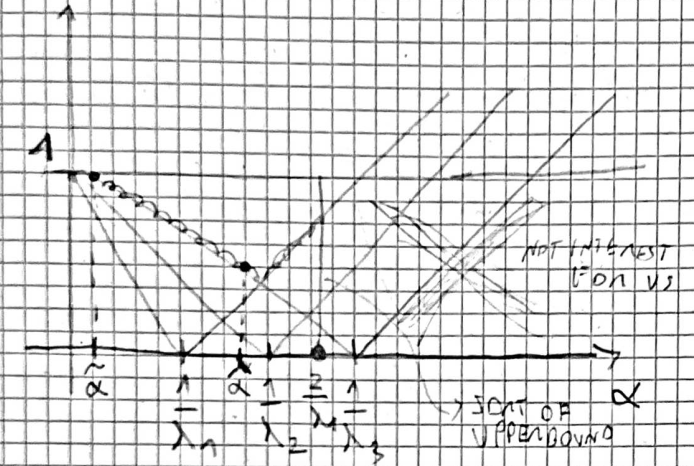
\includegraphics[width=0.9\textwidth]{images/20221118-1.png}
        \end{center}
        Analyzing those 3 plots we can understand why the optimal value is that: we are searching for $\alpha_{opt}$ such that the method is as fast as possible. A method is quicker than the other if its spectral radius is smaller than the second, which means we are finding the value for $\alpha$ such as that the maximum eigenvalue (which is related to the spectral radius) is as small as possible.\\
        On the graph we draw a vertical line in a $\tilde{\alpha}$ which will meet the 3 functions: we will get 3 eigenvalues, we consider the maximum.\\
        Observing the plot, we can see that the maximum eigenvalue is on the branches highlighted, and the $\alpha$ that minimizes the maximum eigenvalue is given by the intersection of the two branches
        $$
        \underlabel{
            1-\alpha\lambda_3
        }{Positive branch}=
        \underlabel{
            \alpha\lambda_1-1
        }{Negative branch}
        \Rightarrow
        \alpha_{opt}=\frac{2}{\lambda_1+\lambda_3}
        $$
        Which is exactly
        $$
        \alpha_{opt}=\frac{2}{\lambda_{\max}(P^{-1}A)+\lambda_{\min}(P^{-1}A)}
        $$
        About the maximum rate of convergence, the spectral radius (with $\lambda_n$ the minimum):
        $$
        \rho(B_{\alpha_{opt}})=1-\alpha_{opt}\lambda_n=
        1-\frac{2\lambda_n}{\lambda_1+\lambda_n}=
        \frac{\lambda_1-\lambda_n}{\lambda_1+\lambda_n}
        $$
        \item Prove that
        $$
        \underlabel{||e^{(k)}||_A}{$x-x^{(k)}$}\leq
        \underlabel{
            \left(
                \frac{
                    K(P^{-1}A)-1
                }{
                    K(P^{-1}A)+1
                }
            \right)^k
        }{
            $<1$
        }||e^{(0)}||_A
        \qquad k\geq 0
        $$
        With $K$ the condition number and $||e||_A$ the energy norm:
        $$
        ||w||_A=\sqrt{w^TAw}\qquad w\leq\mathbb{R}^n
        $$
        We said that the preconditioner matrix $P$ is:
        \begin{itemize}
            \item Nonsingular
            \item Easy to solve, as we have to sovle $Pz^{(k)}=r^{(k)}$
            \item \textbf{Additional condition}, $K(P^{-1}A)$ small
        \end{itemize}
    \end{itemize}

\subsection{Dynamic Richardson Scheme: preconditioned gradient methods}
    If $A$ and $P$ are spd matrices, the dynamic Richardson scheme is convergent \underline{if} (sufficient)
    $$
    \alpha_{k,opt}=\frac{
        \left[z^{(k)}\right]^Tr^{(k)}
    }{
        \left[z^{(k)}\right]^TAz^{(k)}
    }\qquad\forall\,\,k\geq 0,\,\,z^{(k)}=P^{-1}r^{(k)}
    $$
    \textbf{We directly have optimal value for $\alpha$, this method is called preconditioned gradient method}. Moreover, we can exactly prove the same inequality
    $$
    \underlabel{||e^{(k)}||_A}{$x-x^{(k)}$}\leq
    \underlabel{
        \left(
            \frac{
                K(P^{-1}A)-1
            }{
                K(P^{-1}A)+1
            }
        \right)^k
    }{
        $<1$
    }||e^{(0)}||_A
    \qquad k\geq 0
    $$
    Remark: for $P=I$, our optimal recipe for $\alpha$ becomes:
    $$
    \alpha_{k,opt}=\frac{
        \left[r^{(k)}\right]^Tr^{(k)}
    }{
        \left[r^{(k)}\right]^TAr^{(k)}
    }\qquad\forall\,\,k\geq 0,\,\,z^{(k)}=P^{-1}r^{(k)}
    $$
    \textbf{Gradient method}.
    \subsubsection{The algorithm}
    The algorithm has 4 steps
    \begin{center}
        \begin{lstlisting}[language=Matlab, escapeinside=`']
% set intial guess, we can also define associated initial residual
`$x^{(\phi)}\in\mathbb{R}^n\qquad r^{(\phi)}=b-Ax^{(\phi)}$'
for k=0,1,...
    if `$P=I$'
        % got to step 2, 3 steps algorithm in this case
    else
        `1) $Pz^{(k)}=r^{(k)}$'
    `2) $\alpha_{k,opt}=\frac{
        \left[z^{(k)}\right]^Tr^{(k)}
    }{
        \left[z^{(k)}\right]^TAz^{(k)}
    }$'
    `3) $x^{(k+1)}=x^{(k)}+\alpha_{opt,k}z^{(k)}$'
    `4) $r^{(k+1)}=r^{(k)}-\alpha_{opt,k}Az^{(k)}$'
        \end{lstlisting}
    \end{center}
    If stationary, step 2) outside the for cycle
    \begin{center}
        \begin{lstlisting}[language=Matlab, escapeinside=`']
% set intial guess, we can also define associated initial residual
`$x^{(\phi)}\in\mathbb{R}^n\qquad r^{(\phi)}=b-Ax^{(\phi)}$'
`$\alpha_{opt}=...$'
for k=0,1,...
    if `$P=I$'
        % got to step 3, 2 steps algorithm in this case
    else
        `1) $Pz^{(k)}=r^{(k)}$'
    `3) $x^{(k+1)}=x^{(k)}+\alpha_{opt}z^{(k)}$'
    `4) $r^{(k+1)}=r^{(k)}-\alpha_{opt}Az^{(k)}$'
        \end{lstlisting}
    \end{center}
    \subsubsection{Stationary and dynamic: which one is the best}
    Now that we have found the optimal acceleration parameters $\alpha_{opt}$ for both stationary and dynamic cases, which one is better? For stationary we have to find the eigenvalues, but if the matrix is very big this is too demanding, though there are methods to cope with this.

    It is a good idea to prefer dynamic scheme, as in the definition of the acceleration parameter we are using all parameters that are required to be computed for the solution of the system (in the stationary to find the eigenvalues we have to use other parameters unrelated and useless for the solution of our original problem).

    An example
    $$
    \begin{cases}
        2x_1+x_2=1\\
        x_1=3x_2=0
    \end{cases}
    $$
    \begin{center}
        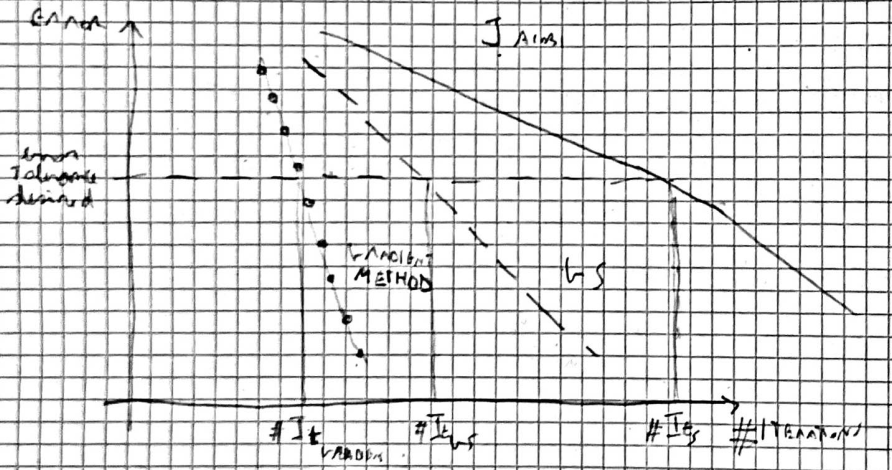
\includegraphics[width=1\textwidth]{images/20221118-2.png}
    \end{center}

    \subsubsection{Proof for the optimal acceleration parameter}
    If $A$ is spd, the solution to our system is: $Ax=b\Leftrightarrow$ equivalent to minimize the quadratic form
    $$Q(x)=\frac{1}{2}x^TAx-x^Tb$$
    as minimizing this quadratic form is solving the gradient w.r.t. 0:
    $$
    \nabla Q(x)=Ax-b=0
    $$
    Note that the quadratic $Q(x)$ is a paraboloid and we are finding its minimum. How to proceed:
    $$
    x^{(k+1)}=x^{(k)}+\gamma_kd^{(k)}
    $$
    with $d^{(k)}$ the direction, \textbf{the steepest descent} and $\gamma_k$ the step size. We choose the steepest direction, so the gradient:
    $$
    d^{(k)}=-\nabla Q(x^{(k)})=b-Ax^{(k)}=r^{(k)}
    $$
    The steepest direction corresponds to the residual. About the step
    $$
    Q\left(
        x^{(k)}+\gamma_kr^{(k)}
    \right)=\tilde{Q}(\gamma_k)
    $$
    Which is the value of $\gamma_k$ that minimizes $Q$? Compute the derivative and impose it to 0
    $$
    \frac{
        d\tilde{Q}
    }{
        d\gamma_k
    }=0
    $$
    $$
    \tilde{Q}(\gamma_k)=Q\left(
        x^{(k)}+\gamma_kr^{(k)}
    \right)=\frac{1}{2}
    \left(
        x^{(k)}+\gamma_kr^{(k)}
    \right)^TA
    \left(
        x^{(k)}+\gamma_kr^{(k)}
    \right)-
    \left(
        x^{(k)}+\gamma_kr^{(k)}
    \right)^Tb
    $$
    Compute the derivative
    $$
    \frac{
        d\tilde{Q}
    }{
        d\gamma_k
    }=
    \left[r^{(k)}\right]^TAx^{(k)}+
    \gamma_k\left[r^{(k)}\right]^TAr^{(k)}-
    \left[r^{(k)}\right]^Tb
    =0
    $$
    $$
    \gamma_k=
    \frac{
        \left[r^{(k)}\right]^T\left(b-Ax^{(k)}\right)
    }{
        \left[r^{(k)}\right]Ar^{(k)}
    }=
    \frac{
        \left[r^{(k)}\right]^Tr^{(k)}
    }{
        \left[r^{(k)}\right]^TAr^{(k)}
    }
    $$
    We found $\alpha_k=P\gamma_k$
    $$
    Pz^{(k)}=r^{(k)}
    $$
    $$
    \alpha^{(k)}=\frac{
        \left[z^{(k)}\right]^Tr^{(k)}
    }{
        \left[z^{(k)}\right]^TAz^{(k)}
    }
    $$

\subsection{Dynamic Richardson Scheme: conjugate gradient method}
    Gradient method can work with Hilbert system (matrix properly preconditioned): conjugate gradient method, 5 steps algorithm that selects a new direction $p^{(k)}$ instead of $d^{(k)}$:
    $$
    \left[p^{(j)}\right]^TAp^{(k+1)}=0
    \qquad j = 0,\cdots,k
    $$
    New direction $A$-orthogonal (or $A$ conjugate) w.r.t. the previous direction.
    \begin{center}
        \begin{lstlisting}[escapeinside=`']
// set intial guess, we can also define associated initial residual
`$x^{(0)}\in\mathbb{R}^n\qquad r^{(0)}=b-Ax^{(0)}$'
for k=0,1,...
    `1) $\alpha_k=...$'
    `2) $x^{(k+1)}=x^{(k)}+\alpha_{k}p^{(k)}$'
    `3) $r^{(k+1)}=r^{(k)}-\alpha_{k}Ap^{(k)}$'
    `4) $\beta_k=...$' // another constant for computing new direction
    `5) $p^{(k+1)}=r^{(k+1)}-\beta_kp^{(k)}$'
        \end{lstlisting}
    \end{center}
    This method wants $A$ spd, also the errors:
    $$
    ||e^{(k)}||_A\leq
    C^k||e^{(0)}||_A
    $$
    $$
    C:=C\left(\sqrt{K(P^{-1}A)}\right)\qquad\text{Depends on sqrt root of condition number of $A$}
    $$
    Consider the Hilbert problem/system, which we remind has a very bad condition number:
    $$
    H_nx_n=b_n
    $$
    \begin{center}        
        \begin{tabular}{c|c|c|c c|c c}
            \textbf{n} & $K(A_n)$ & $\backslash$ & PG & P=D & PCG & P=D\\ \midrule
            4 & & $O(10^{-13})$ & $O(10^{-3})$ & 995 & $O(10^{-2})$ & 3\\ \hline
            6  & &  & & & $O(10^{-2})$ & 4\\ \hline
            8  & &  & & & & 4\\ \hline
            10 & &  & & & & 5\\ \hline
            12 & &  & & & & 5\\ \hline
            14 & & $O(10)$ & $O(10^{-3})$ & 1379 & $O(10^{-3})$ & 5
        \end{tabular}
    \end{center}
    If we can work in an exact arythmetic, this method becomes a direct method.

    \subsection{Stopping Criteria}
    Consider the error estimators: increment and residual
    \subsubsection{Residual}
    $$
    Ax=b
    $$
    $$
    S=r^{(k)}=b-Ax^{(k)}
    $$
    $$
    e^{(k)}=x-x^{(k)}
    $$
    We want to relate the estimator
    $$
    ||e^{(k)}||\qquad S
    $$
    Normalize residual
    $$
    \frac{
        ||e^{(k)}||
    }{
        ||x||
    }
    \leq
    C
    \frac{
        ||r^{(k)}||
    }{
        ||b||
    }
    \leq
    TOL\qquad
    x\neq 0,\,\,b\neq 0
    $$
    The constant $C$ discriminates the reliability or not of our estimator: if it's huge, our estimator is not reliable.\\
    We want to stop at the minimum iteration $kmin$
    $$
    \frac{
        ||e^{(kmin)}||
    }{
        ||x||
    }
    \leq
    C
    \underlabel{
        \frac{
            ||r^{(kmin)}||
        }{
            ||b||
        }
        \leq
        TOL
    }{
        Prove this
    }
    $$
    Remind that
    $$
    \frac{
        ||\delta x=x-\tilde{x}||
    }{
        ||x||
    }
    \leq
    K(A)
    \frac{
        ||r=b-A\tilde{x}||
    }{
        ||b||
    }
    $$
    If we consider $\tilde{x}=x^{(k)}$, we have that:
    $$
    \delta x = e^{(k)}\qquad r = r^{(k)}
    $$
    Which means
    $$
    C=K(A)
    $$
    So regarding the reliability, we have to look at the condition number

    \subsubsection{Increment}
    $$
    Ax=b
    $$
    $$
    S=\delta^{(k)}=x^{(k+1)}-x^{(k)}
    $$
    $$
    kmin\in\mathbb{N}\text{ s.t. }
    ||e^{(kmin)}||\leq C
    \underlabel{
        ||\delta^{(k)}||\leq TOL
    }{Prove this}
    $$
    We start from the below and using triangular inequality:
    $$
    ||e^{(k)}||=||x-x^{(k)}||=
    ||
    \underlabel{
        x-x^{(k+1)}
    }{$e^{(k+1)}$}
    +
    \underlabel{
        x^{(k+1)}-x^{(k)}
    }{$\delta^{(k)}$}
    ||
    \leq
    ||e^{(k+1)}||+||\delta^{(k)}||
    \leq
    \rho(B)||e^{(k)}||+||\delta^{(k)}||
    $$
    $$
    ||e^{(k)}||
    \leq
    \underlabel{
        \frac{
            1
        }{1-\rho(B)}
    }{$C$}
    ||\delta^{(k)}||
    $$
    As we want $C$ as close as possible to 1, we want the spectral radius as close as possible to 0. So increment is a reliable estimator if the spectral radius is very close to 0.\\
    About kmin (minimum number of iterations):
    $$
    e^k=x-x^k
    $$
    $$
    kmin = \frac{
        \log\left[
            \frac{
                \epsilon\cdot(1-||B||_2)
            }{
                ||x^1-x^0||
            }
        \right]
    }{
        \log||B||_2
    }
    $$
    With $\epsilon=TOL$